{ % \renewcommand affects scope within these braces only
\renewcommand{\thechapter}{\arabic{chapter}} % show chapter zero as number (instead of, e.g., roman)
\chapter{Physical Overview of General Relativity}
}

\textsc{In General Relativity}, gravity is no longer a ``force'', but an effect of the \emph{curvature of spacetime}.

\begin{quote}
	\emph{Space tells matter how to move; \\
	\hspace*{1em} Matter tells space how to curve.} \\
	\hspace*{2em} --- Misner, Thorne and Wheeler
\end{quote}

\begin{center}
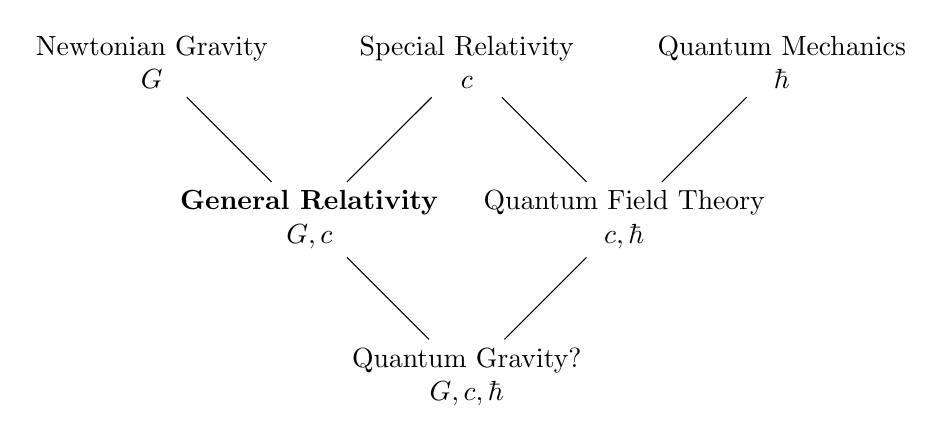
\begin{tikzpicture}[
	scale=2,
	block/.style={
		align=center,
		inner sep=3pt,
	}
]

\node[block] (ng) at (-2,0) {Newtonian Gravity \\ $G$};
\node[block] (sr) at (0,0) {Special Relativity \\ $c$};
\node[block] (qm) at (2,0) {Quantum Mechanics \\ $\hbar$};
\node[block] (gr) at (-1,-1) {\textbf{General Relativity} \\ $G, c$};
\node[block] (qft) at (1,-1) {Quantum Field Theory \\ $c, \hbar$};
\node[block] (qg) at (0,-2) {Quantum Gravity? \\ $G, c, \hbar$};

\draw (ng) -- (gr) -- (sr) -- (qft) -- (qm);
\draw (gr) -- (qg) -- (qft);

\end{tikzpicture}
\end{center}

\noindent
In Newtonian gravity, escape velocity is given by $\frac12mv^2 = \frac{GMm}{R}$.
Hence, gravity is significant if $\frac{v^2}{2} \sim \frac{GM}{R}$.
Special relativity is significant when $v^2 \sim c^2$.
General relativity, at the intersection of the two, is significant when $\frac{c^2}{2} \sim \frac{GM}{R} \iff R \sim \frac{2GM}{c^2}$; this is the \emph{Schwarzschild radius}.
Where the escape velocity coincides with the speed of light, the existence of a \emph{black hole} is implied.